%==============================================================================
% Sjabloon poster bachproef
%==============================================================================
% Gebaseerd op document class `a0poster' door Gerlinde Kettl en Matthias Weiser
% Aangepast voor gebruik aan HOGENT door Jens Buysse en Bert Van Vreckem

\documentclass[a0,portrait]{hogent-poster}

% Info over de opleiding
\course{Bachelorproef}
\studyprogramme{toegepaste informatica}
\academicyear{2024-2025}
\institution{Hogeschool Gent, Valentin Vaerwyckweg 1, 9000 Gent}

% Info over de bachelorproef
\title{Een onderzoek en evaluatie van integratie tools voor ERP optimalisatie en de stroomlijning van bedrijfsprocessen in een snelgroeiende IT-omgeving}
\author{Aron Duym}
\email{aron.duym@student.hogent.be}
\supervisor{Martine Van Audenrode }
\cosupervisor{Laurens Coppens (Axians)}

% Indien ingevuld, wordt deze informatie toegevoegd aan het einde van de
% abstract. Zet in commentaar als je dit niet wilt.
%\specialisation{E-business}
\keywords{ERP optimalisatie, Data integration, BPMS}
%\projectrepo{https://github.com/AronDuym/latex-hogent-bachproef}

\begin{document}

\maketitle

\begin{abstract}
Axians is een IT-provider die begin 2025 de overstap zal maken naar een nieuw ERP-systeem. Deze transitie legt druk op bestaande administratieve processen die momenteel niet optimaal zijn afgestemd op de groei en de interne structuur van het bedrijf. Dit onderzoek richt zich op de vraag welke integratie tool Axians het beste kan ondersteunen bij het stroomlijnen en optimaliseren van hun interne processen. Deze integratie tools worden vervolgens getest en geanalyseerd in een proof of concept waarbij de functionaliteiten en prestaties van iedere tool geëvalueerd worden op basis van een vooropgestelde requirementsanalyse. De verwachte resultaten tonen een rangschikking van de integratie tools op basis van de criteria uit de requirementsanalyse. Deze evaluatie zal Axians voorzien van een duidelijke keuze voor een integratie-oplossing die de interne processen kan optimaliseren en de administratieve belasting kan verminderen. De conclusie van dit onderzoek zal Axians helpen om de best passende integratie tool te selecteren, waardoor de organisatie beter zal kunnen inspelen op interne groei en veranderingen binnen het bedrijf.
\end{abstract}

\begin{multicols}{2} % This is how many columns your poster will be broken into, a portrait poster is generally split into 2 columns

\section{Introductie}

Axians is een IT-provider met zowel software als hardware implementaties en stapt begin 2025 over naar een nieuw ERP pakket. Omwille van interne groei, overnames en organisatorische wijzigingen staan er een aantal manuele en niet-manuele administratieve processen onder druk. Dit zorgt voor fouten en onnodige stress bij medewerkers. 
\vspace{\baselineskip}

Volgens Axians zijn niet alle bedrijfsprocessen en gebruikte tools momenteel goed op elkaar afgestemd. Hierdoor kwam er een verzoek van het bedrijf om onderzoek te doen naar verschillende integraties tools op de markt en deze met elkaar te vergelijken. 
\vspace{\baselineskip}

Dit onderzoek oogt op het ondersteunen van Axians bij het vinden van de optimale integratie tool voor het optimaliseren van het ERP-proces.

\vspace{\baselineskip}

Hierbij luidt de volgende \textbf{onderzoeksvraag} en de bijhorende \textbf{subvragen}:

\vspace{\baselineskip}

Welke integratie tool is het meest geschikt voor Axians om interne processen te optimaliseren en te stroomlijnen tijdens de overstap naar het nieuwe ERP-pakket?

\vspace{\baselineskip}

\textbf{Subvragen:}

Welke integratie tool biedt de meeste mogelijkheden voor uitbreidbaarheid?

Wat zijn de (lange termijn) kosten van elke integratie tool?

Welke integratie tool biedt Axians de meeste functionaliteit?

Welke integratie tool biedt de meeste mogelijkheden voor schaalbaarheid?


\section{Experimenten}

Voor dit onderzoek werd een proof of concept opgesteld dat op een theoretische en praktische manier enkele data integratie tools met elkaar vergelijkt en deze test aan de hand van een requirementsanalyse.

\vspace{\baselineskip}

De eerste stap in dit onderzoek was om samen te zitten met Axians om samen een requirementsanalsye op te stellen en deze te categoriseren aan de hand van de MOSCOW-methode.

\vspace{\baselineskip}

De tweede stap was om eerst een longlist op te stellen met alle mogelijke data integratie tools op de markt, om vervolgens aan de hand van de requirementsanalyse een shortlist op te stellen van data integratie tools die getest zullen worden in de proof of concept. Hierbij werden de integratie tools \textbf{Boomi}, \textbf{Zapier} en \textbf{MicrosoftPA} (Microsoft Power Automate) geselecteerd.

\vspace{\baselineskip}

In de derde en laatste stap worden deze geselecteerde data integratie tools uitgebreid getest aan de hand van de requirementsanalyse. Hierbij wordt bij elke integratie tool een score gegeven tussen 1 en 5 voor elk requirement uit de requirementsanalyse.

\section{Resultaten}

In onderstaande tabel worden de eindresultaten van de hierboven genoemde proof of concept weergegeven. Hier zijn de requirements onderverdeeld per categorie van de MOSCOW-methode en zijn de scores van elke integratie tool naast elkaar geplaatst zodat deze makkelijk te vergelijken zijn.

\begin{center}
  \captionsetup{type=figure}
  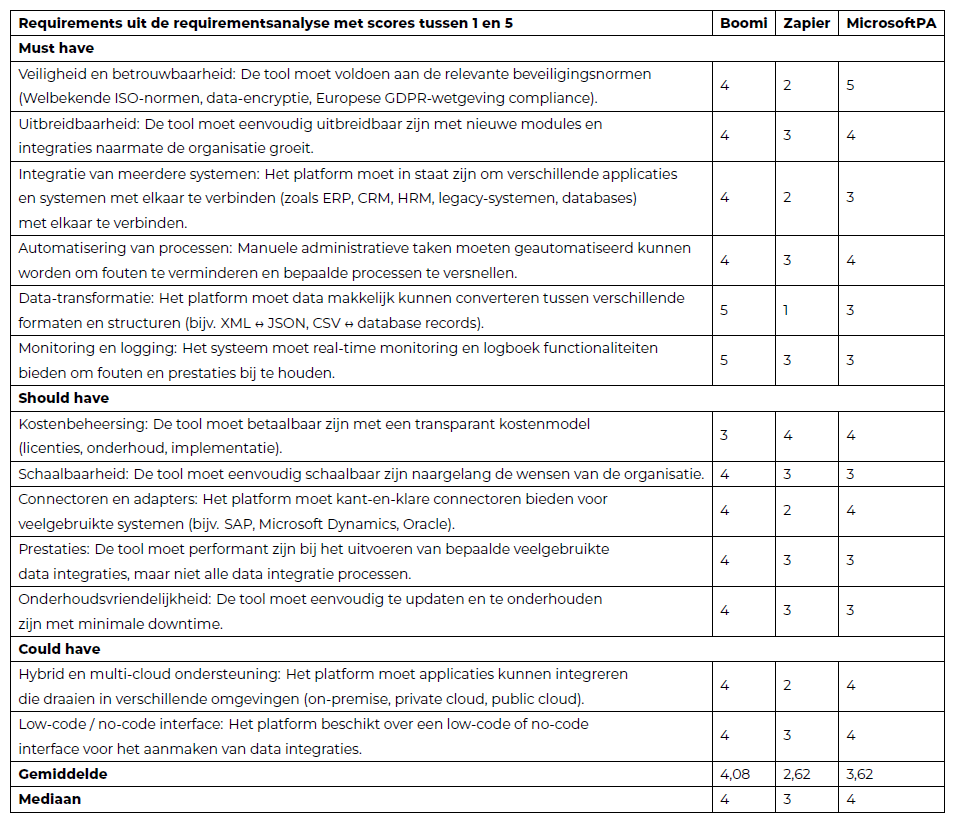
\includegraphics[width=1.0\linewidth]{../poster/images/Eindresultaat.png}
  \captionof{figure}{Eindevaluatie van alle data integratie tools opgedeeld per requirement in de vorm van een tabel}
\end{center}

\section{Conclusies}

Met deze resultaten kan er geconcludeerd worden dat over de algemene lijn, Boomi de beste integratie tool voor Axians lijkt te zijn om op een enterprise-level data integraties aan te kunnen maken. Microsoft Power Automate scoorde ook relatief goed en kan ook dienen als een enterprise-level integratie tool, maar met de focus voor het optimaliseren van bedrijfsprocessen binnen het Microsoft-ecosysteem. Zapier scoorde hierbij het slechtst. Deze integratie tool bleek goed te zijn voor simpele cloud gebaseerde data integraties, maar voldoet niet aan de vereisten van de requirementsanalyse en lijkt ongeschikt om grootschalige enterprise-level data integraties aan te maken.

\section{Toekomstig onderzoek}

Voor de toekomst van dit onderzoek wordt Axians aangeraden om zowel Boomi als Microsoft Power Automate verder te bestuderen. Zo kan het interessant zijn om deze tools op grotere schaal en met complexere data integraties te testen om te zien of deze integratie tools voldoen aan alle eisen van Axians. Tenslotte kan het ook interessant zijn om deze tools te vergelijken met andere integratie tools die niet werden opgenomen in dit onderzoek zoals Mulesoft of APPSeCONNECT, om uiteindelijk een beter oordeel te kunnen maken over welke integratie tool het beste is voor Axians.

\end{multicols}
\end{document}